\section{Databases}

A \textbf{database} is an organized system for storing, retrieving, and managing data. It enables efficient data handling, storage, and access for various applications, from small personal projects to large-scale enterprise solutions. Databases are essential for maintaining consistency, accuracy, and accessibility in data storage. They use structures such as tables to organize data into columns (fields) and rows (records). Two common key elements in databases are \textbf{Primary Keys (PK)} and \textbf{Foreign Keys (FK)}. The Primary Key uniquely identifies each record within a table, ensuring that data remains unique, while the Foreign Key links tables, establishing relationships between them to enforce data integrity.

There are various types of databases, including:
\begin{itemize}
	\item \textbf{Relational Databases} – Organize data into tables and use structured query language (SQL) for data manipulation. Examples include MySQL, PostgreSQL, and SQLite.
	\item \textbf{NoSQL Databases} – Store unstructured data, often in formats like JSON. They are designed for scalability and high performance in handling large datasets, as in MongoDB and Cassandra.
\end{itemize}

\subsection{Entity-Relationship Diagram (ERD)}
The \textbf{Entity-Relationship Diagram (ERD)} is a visual representation of the data model for a system. It illustrates the entities involved, their attributes, and the relationships between them. Each entity corresponds to a table in the database, while attributes represent the fields within those tables. Relationships indicate how entities interact, showcasing cardinality (e.g., one-to-many or many-to-many) and participation (e.g., optional or mandatory). The ERD serves as a crucial tool in the design phase, promoting clear communication about the data structure and its constraints.


\begin{figure}[h]
	\centering
	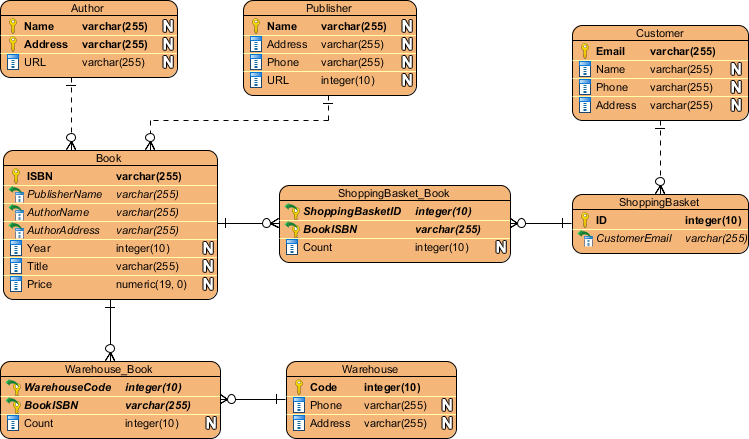
\includegraphics[width=0.9\linewidth]{assets/ch2/ERD}
	\caption{This ERD, adapted from \cite{visual-paradigm}, represents a bookstore database, with entities like Author, Publisher, Book, Warehouse, Customer, and ShoppingBasket. It shows relationships between entities, such as customers adding books to shopping baskets and warehouses storing book inventory, linked by primary and foreign keys.}
	\label{fig:erd}
\end{figure}


\subsection{Structured Query Language (SQL)}
\textbf{SQL (Structured Query Language)} is the standard language used to interact with relational databases. SQL provides commands for data insertion, query, updating, and deletion. It also includes commands for schema creation and modification. Some fundamental SQL commands include:

\begin{itemize}
	\item \texttt{SELECT} for retrieving data,
	\item \texttt{INSERT} for adding new data,
	\item \texttt{UPDATE} for modifying existing data,
	\item \texttt{DELETE} for removing data,
	\item \texttt{CREATE TABLE} for defining new tables,
	\item \texttt{JOIN} for combining data from multiple tables.
\end{itemize}

SQL enables efficient, standardized access to data, supporting complex queries and data manipulation tasks.

\subsection{SQLite3}
\textbf{SQLite3} is a lightweight, serverless, and self-contained relational database engine, commonly used for applications requiring minimal configuration and overhead. Unlike other SQL databases, SQLite does not require a separate server process. Instead, it stores data in a single file, making it highly portable and simple to integrate. SQLite is ideal for embedded systems, mobile apps, and small to medium-scale projects due to its reliability, compact size, and ease of use.
